\documentclass{eeleyes}

\usepackage{physics}

\newcommand\theauthor{Eli Griffiths}

\usepackage{fancyhdr}
\pagestyle{fancy}
\fancyhf{}
\lhead{\theauthor}
\chead{Math 195W}
\rhead{\today}
\rfoot{\thepage}

\author{\theauthor}
\title{\LaTeX \; Assignment 1 \\ \large Math 195W}

\newtcolorbox{problem}{
    colback  = white,
    frame hidden,
    borderline = {1.5pt}{0pt}{black},
    sharp corners,
}

\begin{document}
\maketitle

\begin{theorem}
    Prove the following statement:
    \begin{enumerate}
        \item[]
        If $C$ is a simple closed curve or contour, then $C$ has a bounded inside and unbounded outside.
    \end{enumerate}
\end{theorem}

\begin{proof}
    I mean, just look! Trivial.
    \begin{figure}[h]
        \centering
        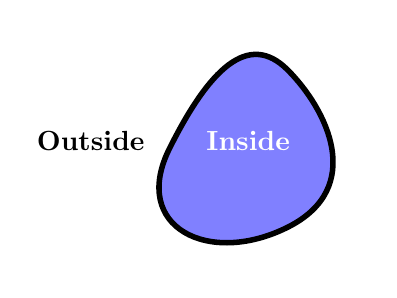
\begin{tikzpicture}[scale=0.5]
            \fill[blue!50, draw=black, line width=2pt] 
            (0,0) .. controls (1,2) and (2,3) .. (3,2)
            .. controls (4,1) and (5,-1) .. (3,-2)
            .. controls (1,-3) and (-1,-2) .. (0,0);
            \node[white] at (2,0.2) {\textbf{Inside}};
            \node at (-2,0.2) {\textbf{Outside}};
        \end{tikzpicture}
    \end{figure}
\end{proof}

\noindent
As one can see, this concept does not need any further investigation because it is so obvious and definitely does not necessitate a complicated proof at all!

\begin{equation}
    \label{eq:tuppers}
    \frac{1}{2} < \left\lfloor \operatorname{mod}\left( \left\lfloor \frac{y}{17} \right\rfloor 2^{-17 \lfloor x \rfloor - \operatorname{mod}(\lfloor y \rfloor, 17))},2 \right) \right\rfloor
\end{equation}

\[
    \mathcal{R}_n(\mathcal{F})=\mathbb{E}_\varepsilon \left[ \sup_{f \in \mathcal{F}} \frac{1}{n} \sum_{i=1}^n \varepsilon_i f(x_i) \right] 
.\]

\[
    f(t) = \frac{\Gamma\qty(\frac{\nu + 1}{2})}{\sqrt{\nu \pi} \Gamma\qty(\frac{\nu}{2})} \left( 1 + \frac{t^2}{\nu} \right)^{-\frac{\nu + 1}{2}}
.\]
If you plot equation \ref{eq:tuppers} which is Tupper's Self Referential Formula and go to
\[
    \begin{array}{r c c c c c c c c c c}
       y= & 960 & 939 & 379 & 918 & 958 & 884 & 971 & 672 & 962 & 127 \\
        & 852 & 754 & 715 & 004 & 339 & 660 & 129 & 306 & 651 & 505 \\
        & 519 & 271 & 702 & 802 & 395 & 266 & 424 & 689 & 642 & 842 \\
        & 174 & 350 & 718 & 121 & 267 & 153 & 782 & 770 & 623 & 355 \\
        & 993 & 237 & 280 & 874 & 144 & 307 & 891 & 325 & 963 & 941 \\
        & 337 & 723 & 487 & 857 & 735 & 749 & 823 & 926 & 629 & 715 \\
        & 517 & 173 & 716 & 995 & 165 & 232 & 890 & 538 & 221 & 612 \\
        & 403 & 238 & 855 & 866 & 184 & 013 & 235 & 585 & 136 & 048 \\
        & 828 & 693 & 337 & 902 & 491 & 454 & 229 & 288 & 667 & 081 \\
        & 096 & 184 & 496 & 091 & 705 & 183 & 454 & 067 & 827 & 731 \\
        & 551 & 705 & 405 & 381 & 627 & 380 & 967 & 602 & 565 & 625 \\
        & 016 & 981 & 482 & 083 & 418 & 783 & 163 & 849 & 115 & 590 \\
        & 225 & 610 & 003 & 652 & 351 & 370 & 343 & 874 & 461 & 848 \\
        & 378 & 737 & 238 & 198 & 224 & 849 & 863 & 465 & 033 & 159 \\
        & 410 & 054 & 974 & 700 & 593 & 138 & 339 & 226 & 497 & 249 \\
        & 461 & 751 & 545 & 728 & 366 & 702 & 369 & 745 & 461 & 014 \\
        & 655 & 997 & 933 & 798 & 537 & 483 & 143 & 786 & 841 & 806 \\
        & 593 & 422 & 227 & 898 & 388 & 722 & 980 & 000 & 748 & 404 \\
        & 719 & & & & & & & & &
    \end{array}
\]
you will see the formula itself plotted.

\end{document}
